

\section{Results}

To evaluate our results, we separated a subset of $13$ frames from the two movies Big Buck Bunny and Elephant Dreams and queried another subset of $100$ disjoint frames (all more than $10$ seconds apart from the queries) as our database.
Our database images have a resolution of $960\times 528$ pixels. We used full resolution for query and half resolution ($480\times 264$) for synthesis.

\newcommand{\SA}[3]{\texttt{#1}\texttt{#2}\texttt{#3}}

We tried $12$ different versions of our algorithm given three parameters:
\begin{itemize}
	\item Transfer type: \texttt{P}atch, \texttt{D}ifference or \texttt{F}low (disparity)
	\item Pyramid type: \texttt{G}aussian or \texttt{L}aplacian
	\item Incremental mode: whether to build incrementally (using the $k$-NNF of the previous scale to initialize the next scale) or not
\end{itemize}

A quantitative evaluation is provided in Table~\ref{tbl:results} showing mean squared error with the true right image.
While most results are still far from perfect, they are all better than using the left frame as is (except for one case).
Furthermore they do not provide a qualitative measurement which would in fact be more useful as it has been shown~\cite{Sawhney01, Stelmach00} that stereo frames needn't be high resolution or very close to ground truth to be acceptable.
The human perception takes care of mixing stereoscopic frames and having one bad frame may often not be perceptible (or at least much less than it appears when looking at the isolated bad frame).
We show a few results synthesis in Figure~\ref{fig:stereo_results} to show that a qualitative measurement would be preferable.

As for our own patch-based disparity computation, we show comparisons with Classic-NL-Fast which we used for disparity transfer in Figure~\ref{fig:disp_results}.
\definecolor{goodcolor}{HTML}{009638}
\newcommand{\best}[1]{\underline{#1}}
\newcommand{\good}{\color{goodcolor}}
\newcommand{\bad}{\color{red}}

\begin{table*}
	\centering
	\begin{tabular}{lc|c|cc|cc|cc}
\bfseries Query & \bfseries Incr & \bfseries Left & \bfseries PG & \bfseries PL & \bfseries DG & \bfseries DL & \bfseries FG & \bfseries FL\\\hline
\texttt{bbb0004} & yes & \best{448.47} & 508.39 & 909.09 & 544.70 & 448.60 & 953.18 & 1167.54 \\
 & no & 448.47 & \good \best{330.71} & 783.08 & \good 473.32 & \good 396.22 & 1001.61 & 1068.16 \\\hline
\texttt{bbb0058} & yes & 426.54 & \good \best{374.43} & 924.03 & 463.75 & 434.48 & 547.73 & 1316.34 \\
 & no & 426.54 & \good \best{330.07} & 782.21 & \good 416.11 & \good 385.33 & 552.99 & 942.46 \\\hline
\texttt{bbb0092} & yes & 234.75 & 1493.95 & 509.31 & 305.32 & \good \best{183.69} & 324.44 & 660.46 \\
 & no & 234.75 & \good \best{34.34} & \good 182.56 & \good 47.63 & \good 39.52 & 355.77 & 565.25 \\\hline
\texttt{bbb0124} & yes & 274.84 & 723.79 & 513.06 & 336.91 & \good  \best{236.69} & 308.30 & 616.81 \\
 & no & 274.84 & \good 67.53 & 448.19 & \good 58.64 & \good \best{51.76} & 294.03 & 568.68 \\\hline
\texttt{bbb0244} & yes & 858.75 & \good \best{795.20} & 1361.74 & 889.92 & 847.25 & 872.70 & 864.40 \\
 & no & 858.75 & \good \best{703.07} & 1212.19 & \good 845.80 & \good 771.82 & 889.23 & 861.11 \\\hline
\texttt{bbb0353} & yes & \best{250.49} & 584.98 & 834.15 & 326.76 & 266.40 & 563.66 & 451.24 \\
 & no & \best{250.49} & 314.41 & 677.53 & 313.59 & 254.26 & 542.74 & 423.58 \\\hline
\texttt{ed0097} & yes & 1649.53 & \good 1130.75 & \good 1132.67 & \good 1646.63 & \good 1565.03 & \good \best{997.70} & \good 1166.23 \\
 & no & 1649.53 & \good \best{1000.37} & \good 1068.22 & \good 1323.11 & \good 1276.36 & \good 1189.43 & \good 1185.89 \\\hline
\texttt{ed0282} & yes & 175.00 & \good 167.14 & 337.87 & 181.94 & \good 151.15 & \good 156.09 & \good \best{133.29} \\
 & no & 175.00 & \good 165.30 & 306.47 & \good 173.29 & \good 148.44 & 182.94 & \good \best{123.91} \\\hline
\texttt{ed0438} & yes & 530.54 & \good 347.67 & \good 508.14 & \good 452.37 & \good 410.18 & \good \best{328.59} & \good 349.03 \\
 & no & 530.54 & \good 375.45 & 540.88 & \good 415.17 & \good 358.42 & \good \best{263.60} & \good 324.05 \\\hline
\texttt{ed0528} & yes & 773.82 & \good 741.03 & \good 681.75 & \good 754.21 & \good 684.74 & \good \best{405.25} & \good 468.93 \\
 & no & 773.82 & \good 513.52 & \good 645.62 & \good 644.25 & \good 579.40 & \good 536.45 & \good \best{449.51} \\\hline
	\end{tabular}
	\caption{Quantitative evaluation of our synthesized frames with the various strategies, the values corresponds to average pixel squared error in $RGB \in [0;255]^3$ space. The first value column includes the error using the left frame as right frame for reference. The columns refer to the algorithm variation: $\textrm{Transfer}\in\{\mbox{\textbf{P}atch}, \mbox{\textbf{D}iff}, \mbox{\textbf{F}low}\}$, $\textrm{Pyramid}\in\{\mbox{\textbf{G}aussian}, \mbox{\textbf{L}aplacian}\}$}
	\label{tbl:results}
\end{table*}

\begin{figure*}
	\centering
	\begin{subfigure}[t]{0.135\textwidth}
		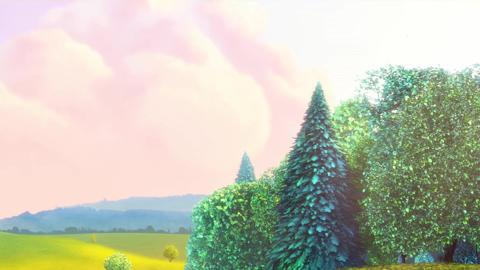
\includegraphics[width=\textwidth]{figures/stereo/bbb_frame-0004-0}\\
		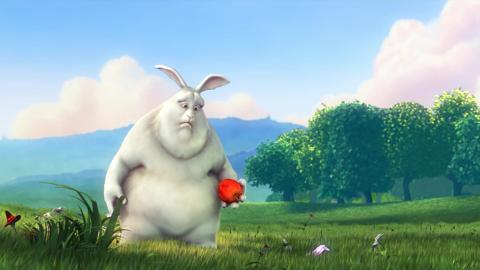
\includegraphics[width=\textwidth]{figures/stereo/bbb_frame-0092-0}\\
		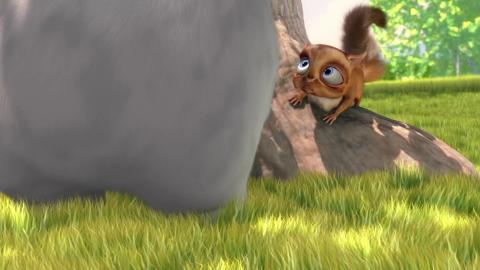
\includegraphics[width=\textwidth]{figures/stereo/bbb_frame-0124-0}\\
		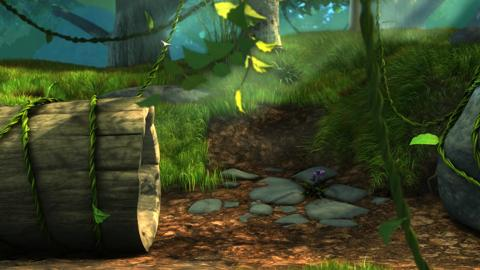
\includegraphics[width=\textwidth]{figures/stereo/bbb_frame-0353-0}\\
		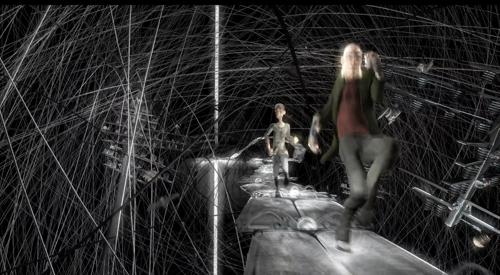
\includegraphics[width=\textwidth]{figures/stereo/ed_frame-0097-0}\\
		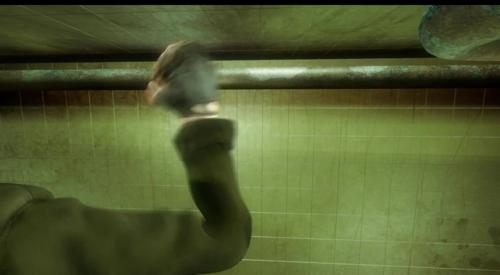
\includegraphics[width=\textwidth]{figures/stereo/ed_frame-0438-0}\\
		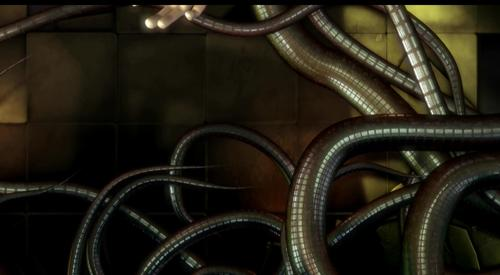
\includegraphics[width=\textwidth]{figures/stereo/ed_frame-0528-0}
		\caption{Ground truth}
	\end{subfigure}
	\begin{subfigure}[t]{0.135\textwidth}
		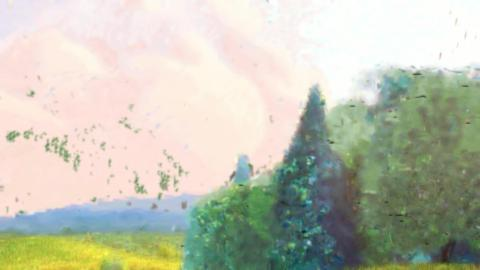
\includegraphics[width=\textwidth]{figures/stereo/bbb_frame-0004-3}\\
		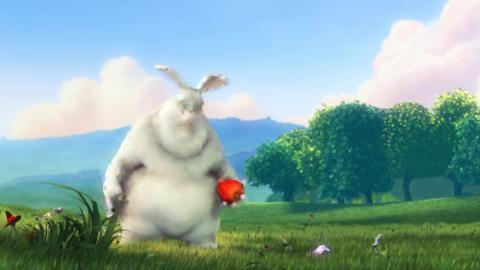
\includegraphics[width=\textwidth]{figures/stereo/bbb_frame-0092-3}\\
		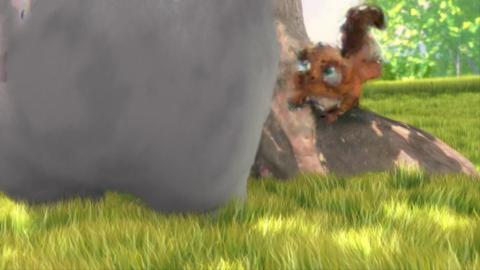
\includegraphics[width=\textwidth]{figures/stereo/bbb_frame-0124-3}\\
		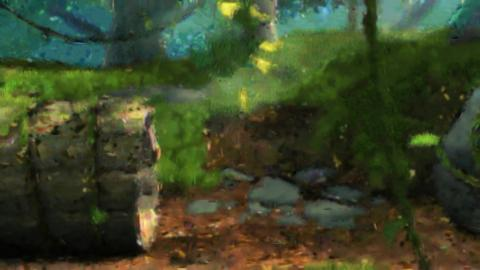
\includegraphics[width=\textwidth]{figures/stereo/bbb_frame-0353-3}\\
		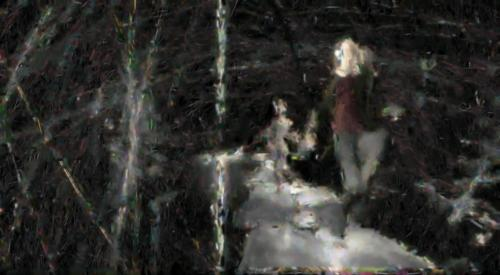
\includegraphics[width=\textwidth]{figures/stereo/ed_frame-0097-3}\\
		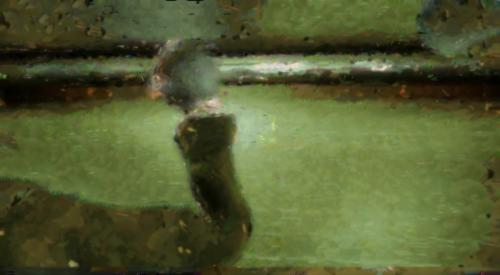
\includegraphics[width=\textwidth]{figures/stereo/ed_frame-0438-3}\\
		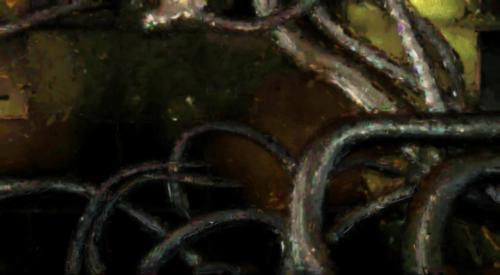
\includegraphics[width=\textwidth]{figures/stereo/ed_frame-0528-3}
		\caption{PG}
	\end{subfigure}
	\begin{subfigure}[t]{0.135\textwidth}
		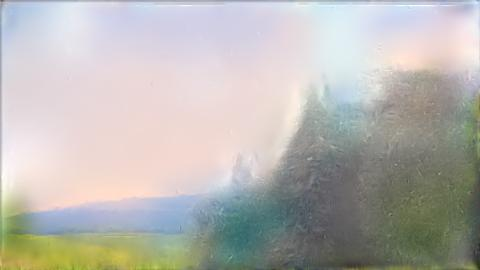
\includegraphics[width=\textwidth]{figures/stereo/bbb_frame-0004-4}\\
		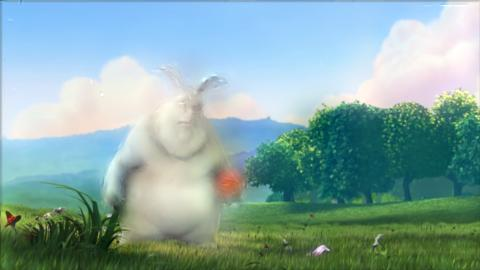
\includegraphics[width=\textwidth]{figures/stereo/bbb_frame-0092-4}\\
		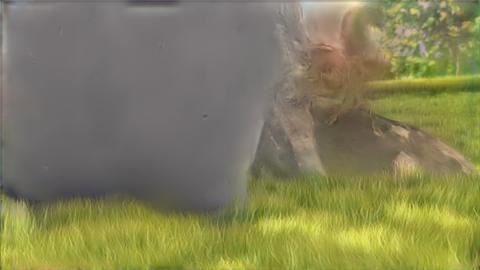
\includegraphics[width=\textwidth]{figures/stereo/bbb_frame-0124-4}\\
		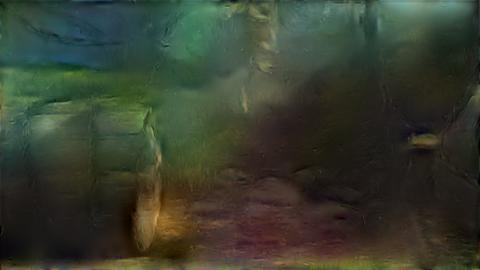
\includegraphics[width=\textwidth]{figures/stereo/bbb_frame-0353-4}\\
		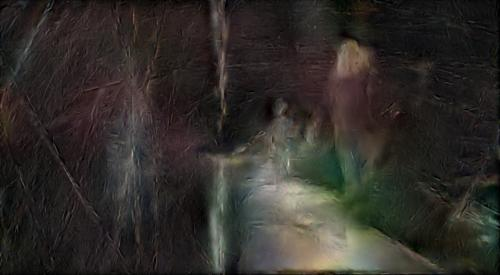
\includegraphics[width=\textwidth]{figures/stereo/ed_frame-0097-4}\\
		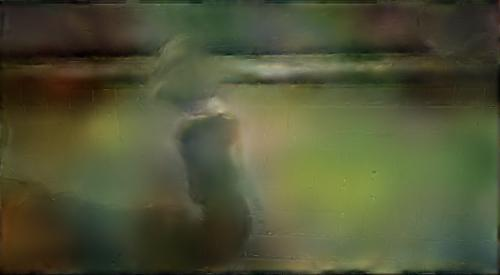
\includegraphics[width=\textwidth]{figures/stereo/ed_frame-0438-4}\\
		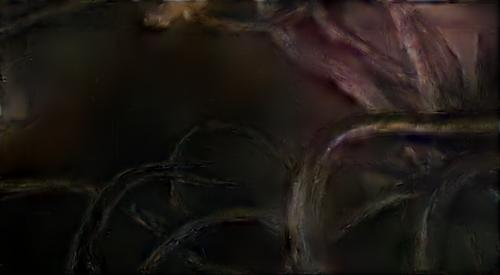
\includegraphics[width=\textwidth]{figures/stereo/ed_frame-0528-4}
		\caption{PL}
	\end{subfigure}
	\begin{subfigure}[t]{0.135\textwidth}
		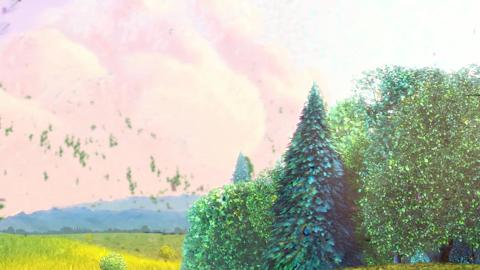
\includegraphics[width=\textwidth]{figures/stereo/bbb_frame-0004-7}\\
		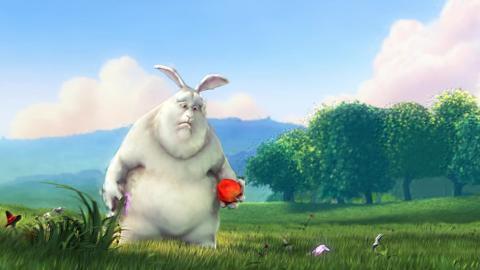
\includegraphics[width=\textwidth]{figures/stereo/bbb_frame-0092-7}\\
		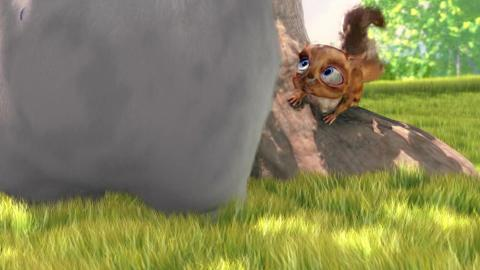
\includegraphics[width=\textwidth]{figures/stereo/bbb_frame-0124-7}\\
		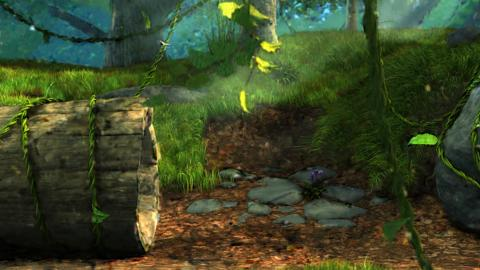
\includegraphics[width=\textwidth]{figures/stereo/bbb_frame-0353-7}\\
		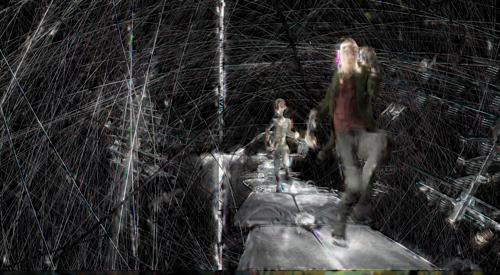
\includegraphics[width=\textwidth]{figures/stereo/ed_frame-0097-7}\\
		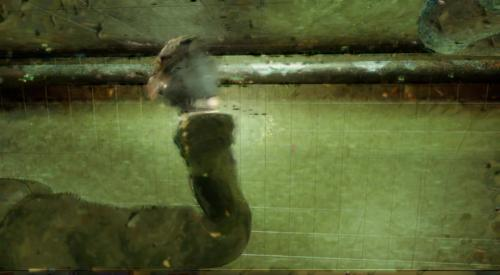
\includegraphics[width=\textwidth]{figures/stereo/ed_frame-0438-7}\\
		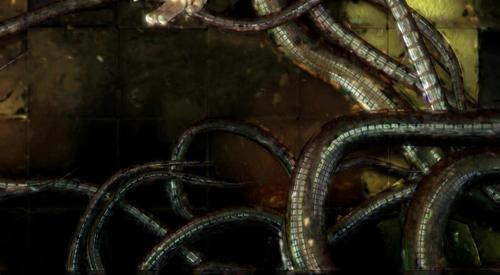
\includegraphics[width=\textwidth]{figures/stereo/ed_frame-0528-7}
		\caption{DG}
	\end{subfigure}
	\begin{subfigure}[t]{0.135\textwidth}
		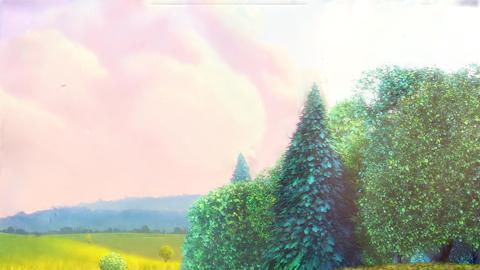
\includegraphics[width=\textwidth]{figures/stereo/bbb_frame-0004-8}\\
		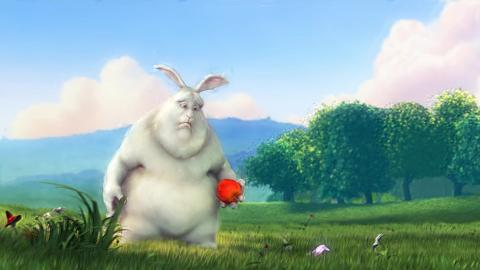
\includegraphics[width=\textwidth]{figures/stereo/bbb_frame-0092-8}\\
		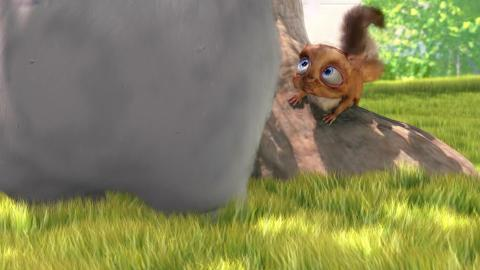
\includegraphics[width=\textwidth]{figures/stereo/bbb_frame-0124-8}\\
		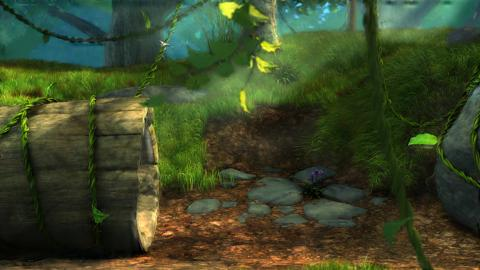
\includegraphics[width=\textwidth]{figures/stereo/bbb_frame-0353-8}\\
		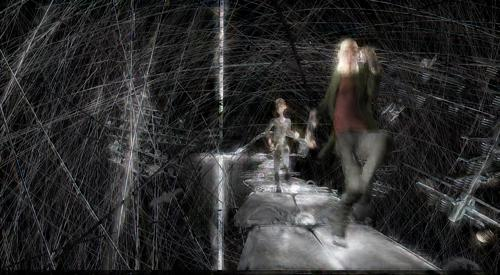
\includegraphics[width=\textwidth]{figures/stereo/ed_frame-0097-8}\\
		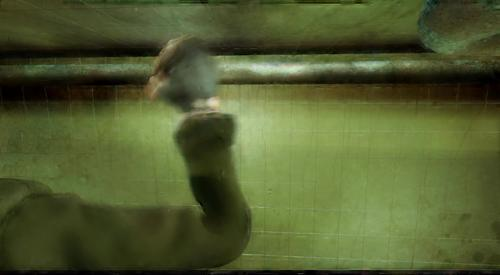
\includegraphics[width=\textwidth]{figures/stereo/ed_frame-0438-8}\\
		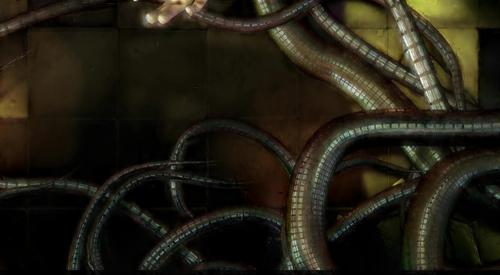
\includegraphics[width=\textwidth]{figures/stereo/ed_frame-0528-8}
		\caption{DL}
	\end{subfigure}
	\begin{subfigure}[t]{0.135\textwidth}
		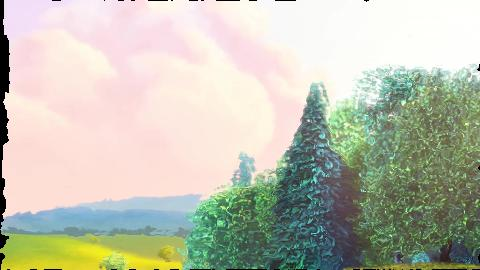
\includegraphics[width=\textwidth]{figures/stereo/bbb_frame-0004-11}\\
		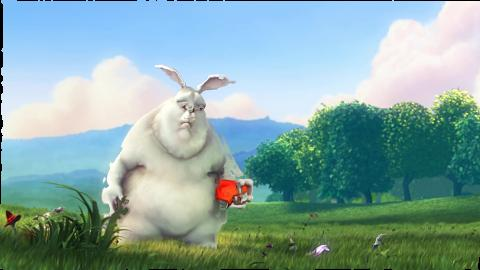
\includegraphics[width=\textwidth]{figures/stereo/bbb_frame-0092-11}\\
		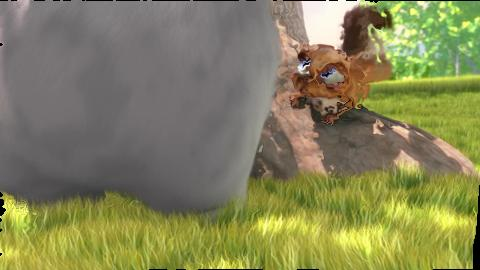
\includegraphics[width=\textwidth]{figures/stereo/bbb_frame-0124-11}\\
		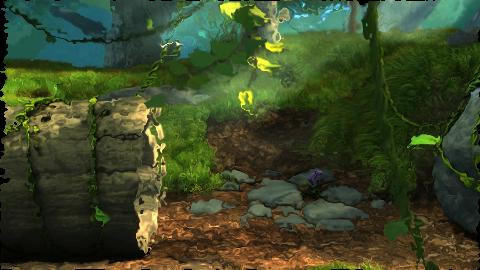
\includegraphics[width=\textwidth]{figures/stereo/bbb_frame-0353-11}\\
		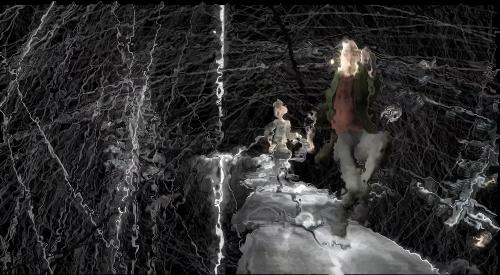
\includegraphics[width=\textwidth]{figures/stereo/ed_frame-0097-11}\\
		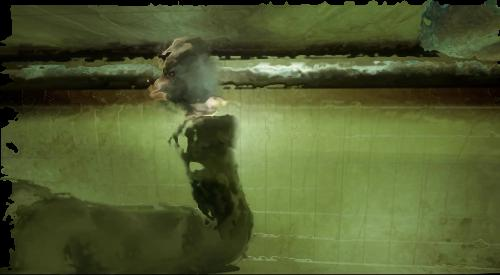
\includegraphics[width=\textwidth]{figures/stereo/ed_frame-0438-11}\\
		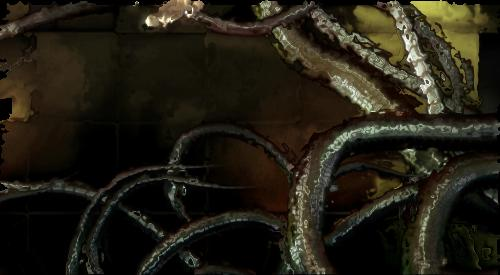
\includegraphics[width=\textwidth]{figures/stereo/ed_frame-0528-11}
		\caption{FG}
	\end{subfigure}
	\begin{subfigure}[t]{0.135\textwidth}
		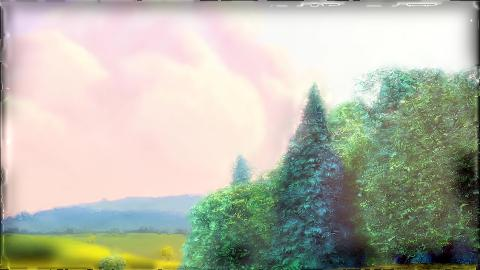
\includegraphics[width=\textwidth]{figures/stereo/bbb_frame-0004-12}\\
		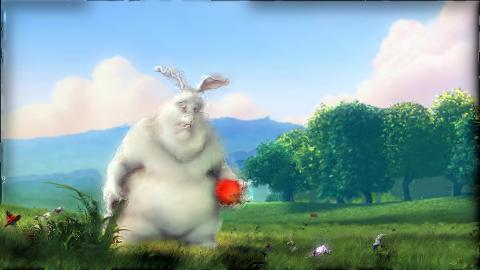
\includegraphics[width=\textwidth]{figures/stereo/bbb_frame-0092-12}\\
		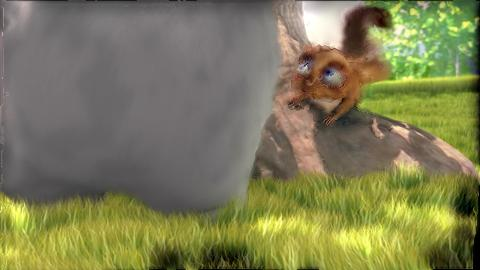
\includegraphics[width=\textwidth]{figures/stereo/bbb_frame-0124-12}\\
		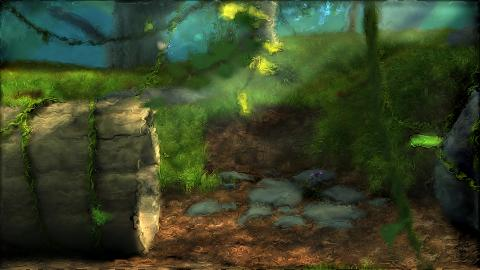
\includegraphics[width=\textwidth]{figures/stereo/bbb_frame-0353-12}\\
		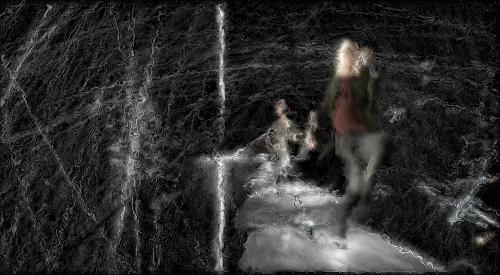
\includegraphics[width=\textwidth]{figures/stereo/ed_frame-0097-12}\\
		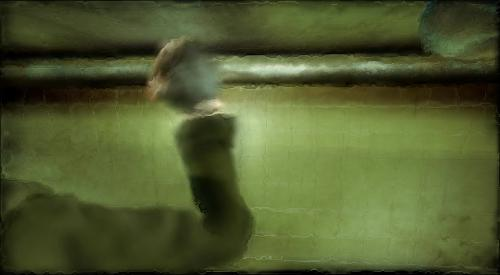
\includegraphics[width=\textwidth]{figures/stereo/ed_frame-0438-12}\\
		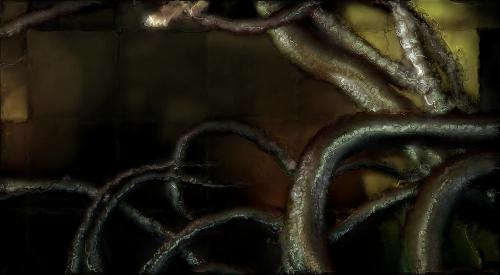
\includegraphics[width=\textwidth]{figures/stereo/ed_frame-0528-12}
		\caption{FL}
	\end{subfigure}
	\caption{Examples of non-incremental stereo analogy results: from top to bottom, \texttt{bbb\_frame-0004}, \texttt{bbb\_frame-0092}, \texttt{bbb\_frame-0124}, \texttt{bbb\_frame-0353}, \texttt{ed\_frame-0097}, \texttt{ed\_frame-0438}, \texttt{ed\_frame-0528}}
	\label{fig:stereo_results}
\end{figure*}

\begin{figure*}
	\centering
	\begin{subfigure}[t]{0.24\textwidth}
		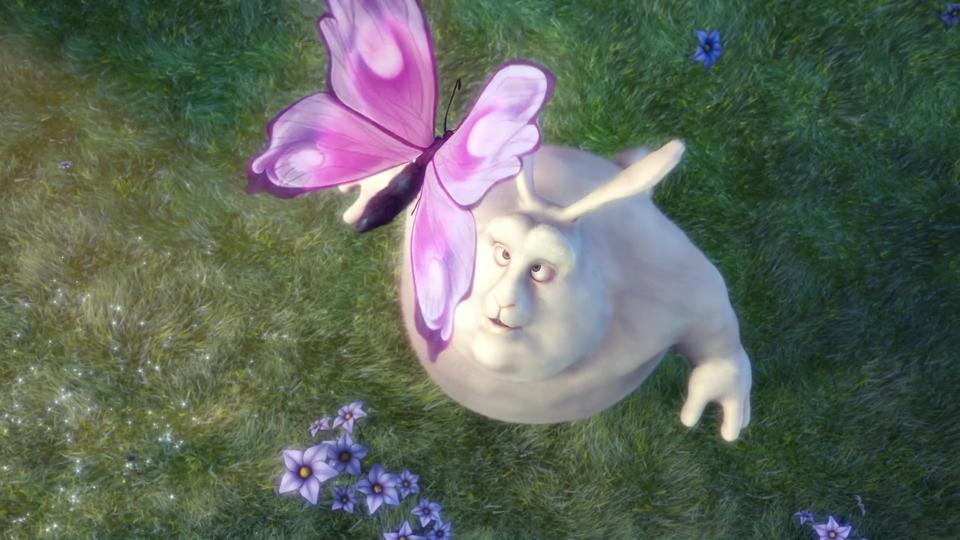
\includegraphics[width=\textwidth]{figures/frames/left/frame-0076}\\
		\includegraphics[width=\textwidth]{figures/frames/left/frame-0391}
		\caption{Left frame}
	\end{subfigure}
	\begin{subfigure}[t]{0.24\textwidth}
		\includegraphics[width=\textwidth]{figures/frames/right/frame-0076}\\
		\includegraphics[width=\textwidth]{figures/frames/right/frame-0391}
		\caption{Right frame}
	\end{subfigure}
	\begin{subfigure}[t]{0.24\textwidth}
		\includegraphics[width=\textwidth]{figures/classicnlp/frame-0076}\\
		\includegraphics[width=\textwidth]{figures/classicnlp/frame-0391}
		\caption{Classic-NL-Fast}
	\end{subfigure}
	\begin{subfigure}[t]{0.24\textwidth}
		\includegraphics[width=\textwidth]{figures/uv/frame-0076}\\
		\includegraphics[width=\textwidth]{figures/uv/frame-0391}
		\caption{Our patch-based disparity}
	\end{subfigure}
	\caption{A few examples of disparity results}
	\label{fig:disp_results}
\end{figure*}